%!TEX root = Uno-Dokumentation.tex

\chapter{Software}

\section{Grundlegender Aufbau}
In diesem Kapitel wird auf den Aufbau der gesamten Software eingegangen und soll einen Überblick über das Projekt geben. Abbildung \ref{fig:aufbau} zeigt die Menüführung der Software als Blockdiagramm. 
\begin{figure}[h]
	\begin{center}
		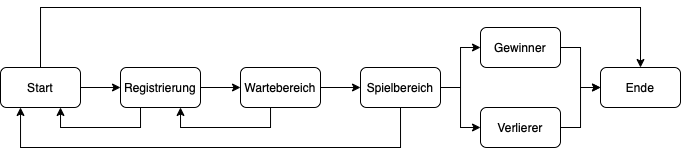
\includegraphics[width=\linewidth]{Uno_Pages.png}
		\caption{Blockdiagramm Software-Aufbau}
		\label{fig:aufbau}
	\end{center}
\end{figure}
Wird die Software gestartet, so wird die Startseite aufgerufen. Hier kann der Spieler das Spiel beenden, starten oder die Spielregeln einsehen. Wird das Spiel gestartet öffnet sich die Registrierungsseite. Hier wird der Spieler dazu aufgefordert seinen Namen einzugeben. Der Name wird dazu verwendet, um später im Spiel zu identifizieren welcher Spieler gerade am Zug ist. Für die Eingabe des Namens steht ein Textfeld zur Verfügung, welches auf maximal 20 einzugebende Zeichen begrenzt ist. Startet der Spieler das Spiel, so wird standardmäßig versucht eine Verbindung zu einem bestehenden Server aufzubauen. Wird jedoch ein Häkchen auf der Registrierungsseite gesetzt, so kann ein neuer Server gestartet werden. Nach der Registrierung wird der Spieler in einen Wartebereich geleitet. Dort wird auf die anderen drei Spieler gewartet. Entsprechende Benutzerrückmeldungen zeigen den aktuellen Status der Netzwerkverbindung und neu verbundene oder getrennte Spieler. Der Wartebereich wird automatisch verlassen, wenn vier Spieler erfolgreich mit dem Server verbunden sind. Ist dies der Fall, öffnet sich der Spielbereich. In diesem Bereich wird das Spiel gespielt. Je nach dem ob der Spieler die Runde gewinnt oder verliert, öffnet sich eine entsprechende Seite, auf der das Ergebnis gezeigt wird. Bei den Spielern, die verloren haben, wird der Name des Spielers gezeigt der die Runde gewonnen hat. Die Software kann an diesem Punkt nur noch beendet werden. Um eine neue Runde zu starten muss auch die Software neu gestartet werden.
\section{Klassen}
\subsection{Player}
\subsection{Card / CardStack}
Die Spielkarten spielen eine essentielle Rolle. Aus diesem Grund werden zwei Klassen für den Umgang mit den einzelnen Karten (\textit{Card}) und einem Kartenstapel (\textit{CardStack}) verwendet. Zunächst wird die Klasse \textit{Card} für eine einzelne Karte betrachtet. Wie in Kapitel \ref{ch:bedingungen} beschrieben, werden nur einfache Karten programmiert. Sie bestehen aus einer Farbe, repräsentiert durch einen ganzzahligen Zahlenwert zwischen null und drei und einer Zahl zwischen null und neun. Codeausschnitt \ref{code:card} zeigt einen Ausschnitt der Klasse \textit{Card}. Weitere Attribute werden für eine einfache Karte nicht benötigt. Die Klasse kann jedoch erweitert werden um Spezialkarten repräsentieren zu können.
\begin{lstlisting}[label={code:card}, caption={Codeausschnitt Klasse \textit{Card}}]
	public class Card
	{
		public int number;
		public int color;
		
		public Card(int number, int color)
		{
			this.number = number;
			this.color = color;
		}
	}
\end{lstlisting}
Codeausschnitt \ref{code:stack} zeigt den grundsätzlichen Aufbau der \textit{CardStack}-Klasse. Ein Karten-Stapel (CardStack) besteht aus einer Liste (\textit{Cards}) mit Elementen des Typs \textit{Card}. Zu beginn eines Spiels werden mithilfe der Methode \textit{createAllCards()} alle möglichen Spielkarten, wie in Kapitel \ref{ch:karten} beschrieben zu der Liste \textit{Cards} hinzugefügt. Um eine Karte zu ziehen, wird die Methode \textit{getRandomCard()} verwendet. Die Methode gibt eine zufällig gewählte Karte zurück und entfernt sie aus dem Stapel. Mithilfe der Methode \textit{returnCard(int index)} kann eine Karte an einer spezifischen Stelle des Stapels erhalten werden. Ein Karte kann dem Stapel mit der Methode \textit{AddCard(Card add)} hinzugefügt und mit \textit{RemoveCard(Card rem)} entfernt werden. Eine Karte kann nur entfernt werden, wenn sie in der Liste vorhanden ist. Ist die Karte nicht in der Liste vorhanden, so ist der Rückgabewert der Methode \textit{null}. Die Anzahl der Karten im Stapel wird mit der Methode \textit{getCounter()} zurückgegeben.
\begin{lstlisting}[label={code:stack}, caption={Codeausschnitt Klasse \textit{CardStack}}]
	public class CardStack
	{
		public List<Card> Cards { get; set; }
		public CardStack()
		{
			this.Cards = new List<Card>();
		}
		
		public void createAllCards();
		public Card getRandomCard();
		public Card returnCard(int index);
		public void AddCard(Card add);
		public Card RemoveCard(Card rem);
		public int getCounter();
	}
\end{lstlisting}
\subsection{Client}
\subsection{GameServer}
Der \textit{GameServer} ist das Herzstück der Anwendung. Er verarbeitet jegliche Spiellogik und Anfragen von Clients aller Spieler. Im folgenden wird genauer auf die Klasse eingegangen.\\
Für die Server-Client-Verbindung wird ein sogenanntes \textit{NuGet-Paket} verwendet, welches compilierten Code enthält, der in externen Projekten verwendet werden kann \cite{NuGet}. Im Rahmen dieser Arbeit wird das \textit{SuperSimpleTCP}-Paket verwendet. Es enthält alle Klassen und Methoden, um einfache Server-Client-Verbindungen über das TCP-Protokoll herzustellen.\\
%TODO TCP acro
Codeausschnitt \ref{code:gameserver} zeigt einen Ausschnitt der \textit{GameServer}-Klasse. Es handelt sich dabei um eine statische Klasse, da der Server zu jedem Zeitpunkt verfügbar sein muss und nur eine einzige Instanz der Klasse benötigt wird. Der Klassen-Member \textit{server} beinhaltet alle Server-Funktionalitäten. Mit der Methode \textit{StartServer()} wird ein neuer Server gestartet und die Event-Methoden in Zeile 11 - 13 an die entsprechenden Server-Events angefügt. Wird nun ein Datenpaket empfangen, so wird ein neuer Thread gestartet, indem das eingehende Datenpaket entsprechend seines Inhalts verarbeitet wird. Die private Klasse \textit{RxMsg} dient zur Verarbeitung der Nachricht. Mit der Methode \textit{Stop()} werden aktive Verbindungen getrennt und der Server gestoppt. Wird eine neue Verbindung eines Clients zum Server festgestellt, wird der Client dazu aufgefordert den auf der Registierungsseite eingegebenen Namen zum Server zu schicken. Es wird geprüft, ob der Name von einem anderen schon verbundenen Spieler genutzt wird. Ist dies der Fall, so wird an den Namen ein Ausrufezeichen angehängt und an den Client zurückgeschickt. Nach der Namensprüfung wird der Spieler zu der Liste \textit{AllPlayers} hinzugefügt. Wird eine bestehende Verbindung getrennt, wird der entsprechende Spieler wieder von der Liste entfernt. Bei jeder neuen Verbindung wird geprüft, ob die Zielanzahl von vier Spielern erreicht ist, also ob die Liste \textit{AllPlayers} vier Elemente enthält. Ist dies der Fall wird eine Nachricht mithilfe der Methode \textit{serverBroadcast()} an alle verbundenen Clients gesendet, die den Start des Spiels signalisiert. Daraufhin wird serverseitig das Spiel gestartet, d.h. alle Spielkarten werden generiert und in der Liste \textit{AllCards} gespeichert, eine zufällige Karte aus \textit{AllCrards} auf den in der Tischmitte liegenden Stapel (\textit{MiddleStack}) verschoben und jeweils sieben Karten an jeden Client gesendet. Die Variable \textit{activePlayer} steht für den Spieler, der gerade am Zug ist.
\begin{lstlisting}[label={code:gameserver}, caption={Codeausschnitt Klasse \textit{GameServer}}]
	static class GameServer
	{
		static private SimpleTcpServer server;
		static private CardStack AllCards;
		static private CardStack MiddleStack;
		static private List<Player> AllPlayers = new List<Player>();
		static private int activePlayer = 0;
		
		static public bool StartServer();
		
		private static void Events_DataReceived(object? sender, DataReceivedEventArgs e);
		private static void Events_ClientDisconnected(object? sender, ConnectionEventArgs e);
		private static void Events_ClientConnected(object? sender, ConnectionEventArgs e);
		
		public static void serverBroadcast(string msg);
		public static void Stop();
		public static void StartGame();
		private static void removePlayer(string IpPort);
		public static bool isActive();
		
		private class RxMsg;
		{
			public string addPlayer(string name, string IpPort);
			public void removePlayer(string IpPort);
			private string CheckDuplicateNames(string name);
			private bool checkMovePossibility(int number, int color);
		}
	}
\end{lstlisting}